% Options for packages loaded elsewhere
% Options for packages loaded elsewhere
\PassOptionsToPackage{unicode}{hyperref}
\PassOptionsToPackage{hyphens}{url}
\PassOptionsToPackage{dvipsnames,svgnames,x11names}{xcolor}
%
\documentclass[
  letterpaper,
  DIV=11,
  numbers=noendperiod]{scrreprt}
\usepackage{xcolor}
\usepackage{amsmath,amssymb}
\setcounter{secnumdepth}{5}
\usepackage{iftex}
\ifPDFTeX
  \usepackage[T1]{fontenc}
  \usepackage[utf8]{inputenc}
  \usepackage{textcomp} % provide euro and other symbols
\else % if luatex or xetex
  \usepackage{unicode-math} % this also loads fontspec
  \defaultfontfeatures{Scale=MatchLowercase}
  \defaultfontfeatures[\rmfamily]{Ligatures=TeX,Scale=1}
\fi
\usepackage{lmodern}
\ifPDFTeX\else
  % xetex/luatex font selection
\fi
% Use upquote if available, for straight quotes in verbatim environments
\IfFileExists{upquote.sty}{\usepackage{upquote}}{}
\IfFileExists{microtype.sty}{% use microtype if available
  \usepackage[]{microtype}
  \UseMicrotypeSet[protrusion]{basicmath} % disable protrusion for tt fonts
}{}
\makeatletter
\@ifundefined{KOMAClassName}{% if non-KOMA class
  \IfFileExists{parskip.sty}{%
    \usepackage{parskip}
  }{% else
    \setlength{\parindent}{0pt}
    \setlength{\parskip}{6pt plus 2pt minus 1pt}}
}{% if KOMA class
  \KOMAoptions{parskip=half}}
\makeatother
% Make \paragraph and \subparagraph free-standing
\makeatletter
\ifx\paragraph\undefined\else
  \let\oldparagraph\paragraph
  \renewcommand{\paragraph}{
    \@ifstar
      \xxxParagraphStar
      \xxxParagraphNoStar
  }
  \newcommand{\xxxParagraphStar}[1]{\oldparagraph*{#1}\mbox{}}
  \newcommand{\xxxParagraphNoStar}[1]{\oldparagraph{#1}\mbox{}}
\fi
\ifx\subparagraph\undefined\else
  \let\oldsubparagraph\subparagraph
  \renewcommand{\subparagraph}{
    \@ifstar
      \xxxSubParagraphStar
      \xxxSubParagraphNoStar
  }
  \newcommand{\xxxSubParagraphStar}[1]{\oldsubparagraph*{#1}\mbox{}}
  \newcommand{\xxxSubParagraphNoStar}[1]{\oldsubparagraph{#1}\mbox{}}
\fi
\makeatother


\usepackage{longtable,booktabs,array}
\usepackage{calc} % for calculating minipage widths
% Correct order of tables after \paragraph or \subparagraph
\usepackage{etoolbox}
\makeatletter
\patchcmd\longtable{\par}{\if@noskipsec\mbox{}\fi\par}{}{}
\makeatother
% Allow footnotes in longtable head/foot
\IfFileExists{footnotehyper.sty}{\usepackage{footnotehyper}}{\usepackage{footnote}}
\makesavenoteenv{longtable}
\usepackage{graphicx}
\makeatletter
\newsavebox\pandoc@box
\newcommand*\pandocbounded[1]{% scales image to fit in text height/width
  \sbox\pandoc@box{#1}%
  \Gscale@div\@tempa{\textheight}{\dimexpr\ht\pandoc@box+\dp\pandoc@box\relax}%
  \Gscale@div\@tempb{\linewidth}{\wd\pandoc@box}%
  \ifdim\@tempb\p@<\@tempa\p@\let\@tempa\@tempb\fi% select the smaller of both
  \ifdim\@tempa\p@<\p@\scalebox{\@tempa}{\usebox\pandoc@box}%
  \else\usebox{\pandoc@box}%
  \fi%
}
% Set default figure placement to htbp
\def\fps@figure{htbp}
\makeatother





\setlength{\emergencystretch}{3em} % prevent overfull lines

\providecommand{\tightlist}{%
  \setlength{\itemsep}{0pt}\setlength{\parskip}{0pt}}



 


\KOMAoption{captions}{tableheading}
\makeatletter
\@ifpackageloaded{bookmark}{}{\usepackage{bookmark}}
\makeatother
\makeatletter
\@ifpackageloaded{caption}{}{\usepackage{caption}}
\AtBeginDocument{%
\ifdefined\contentsname
  \renewcommand*\contentsname{Table of contents}
\else
  \newcommand\contentsname{Table of contents}
\fi
\ifdefined\listfigurename
  \renewcommand*\listfigurename{List of Figures}
\else
  \newcommand\listfigurename{List of Figures}
\fi
\ifdefined\listtablename
  \renewcommand*\listtablename{List of Tables}
\else
  \newcommand\listtablename{List of Tables}
\fi
\ifdefined\figurename
  \renewcommand*\figurename{Figure}
\else
  \newcommand\figurename{Figure}
\fi
\ifdefined\tablename
  \renewcommand*\tablename{Table}
\else
  \newcommand\tablename{Table}
\fi
}
\@ifpackageloaded{float}{}{\usepackage{float}}
\floatstyle{ruled}
\@ifundefined{c@chapter}{\newfloat{codelisting}{h}{lop}}{\newfloat{codelisting}{h}{lop}[chapter]}
\floatname{codelisting}{Listing}
\newcommand*\listoflistings{\listof{codelisting}{List of Listings}}
\makeatother
\makeatletter
\makeatother
\makeatletter
\@ifpackageloaded{caption}{}{\usepackage{caption}}
\@ifpackageloaded{subcaption}{}{\usepackage{subcaption}}
\makeatother
\usepackage{bookmark}
\IfFileExists{xurl.sty}{\usepackage{xurl}}{} % add URL line breaks if available
\urlstyle{same}
\hypersetup{
  pdftitle={Jonathan Kenan Budianto},
  pdfauthor={13523139 Jonathan Kenan Budianto},
  colorlinks=true,
  linkcolor={blue},
  filecolor={Maroon},
  citecolor={Blue},
  urlcolor={Blue},
  pdfcreator={LaTeX via pandoc}}


\title{Jonathan Kenan Budianto}
\usepackage{etoolbox}
\makeatletter
\providecommand{\subtitle}[1]{% add subtitle to \maketitle
  \apptocmd{\@title}{\par {\large #1 \par}}{}{}
}
\makeatother
\subtitle{Portfolio Asesmen II-2100 KIPP}
\author{13523139 Jonathan Kenan Budianto}
\date{2025-10-28}
\begin{document}
\maketitle

\renewcommand*\contentsname{Table of contents}
{
\hypersetup{linkcolor=}
\setcounter{tocdepth}{2}
\tableofcontents
}

\bookmarksetup{startatroot}

\chapter*{Salam Kenal Semua!}\label{salam-kenal-semua}
\addcontentsline{toc}{chapter}{Salam Kenal Semua!}

\markboth{Salam Kenal Semua!}{Salam Kenal Semua!}

\begin{figure}[H]

{\centering 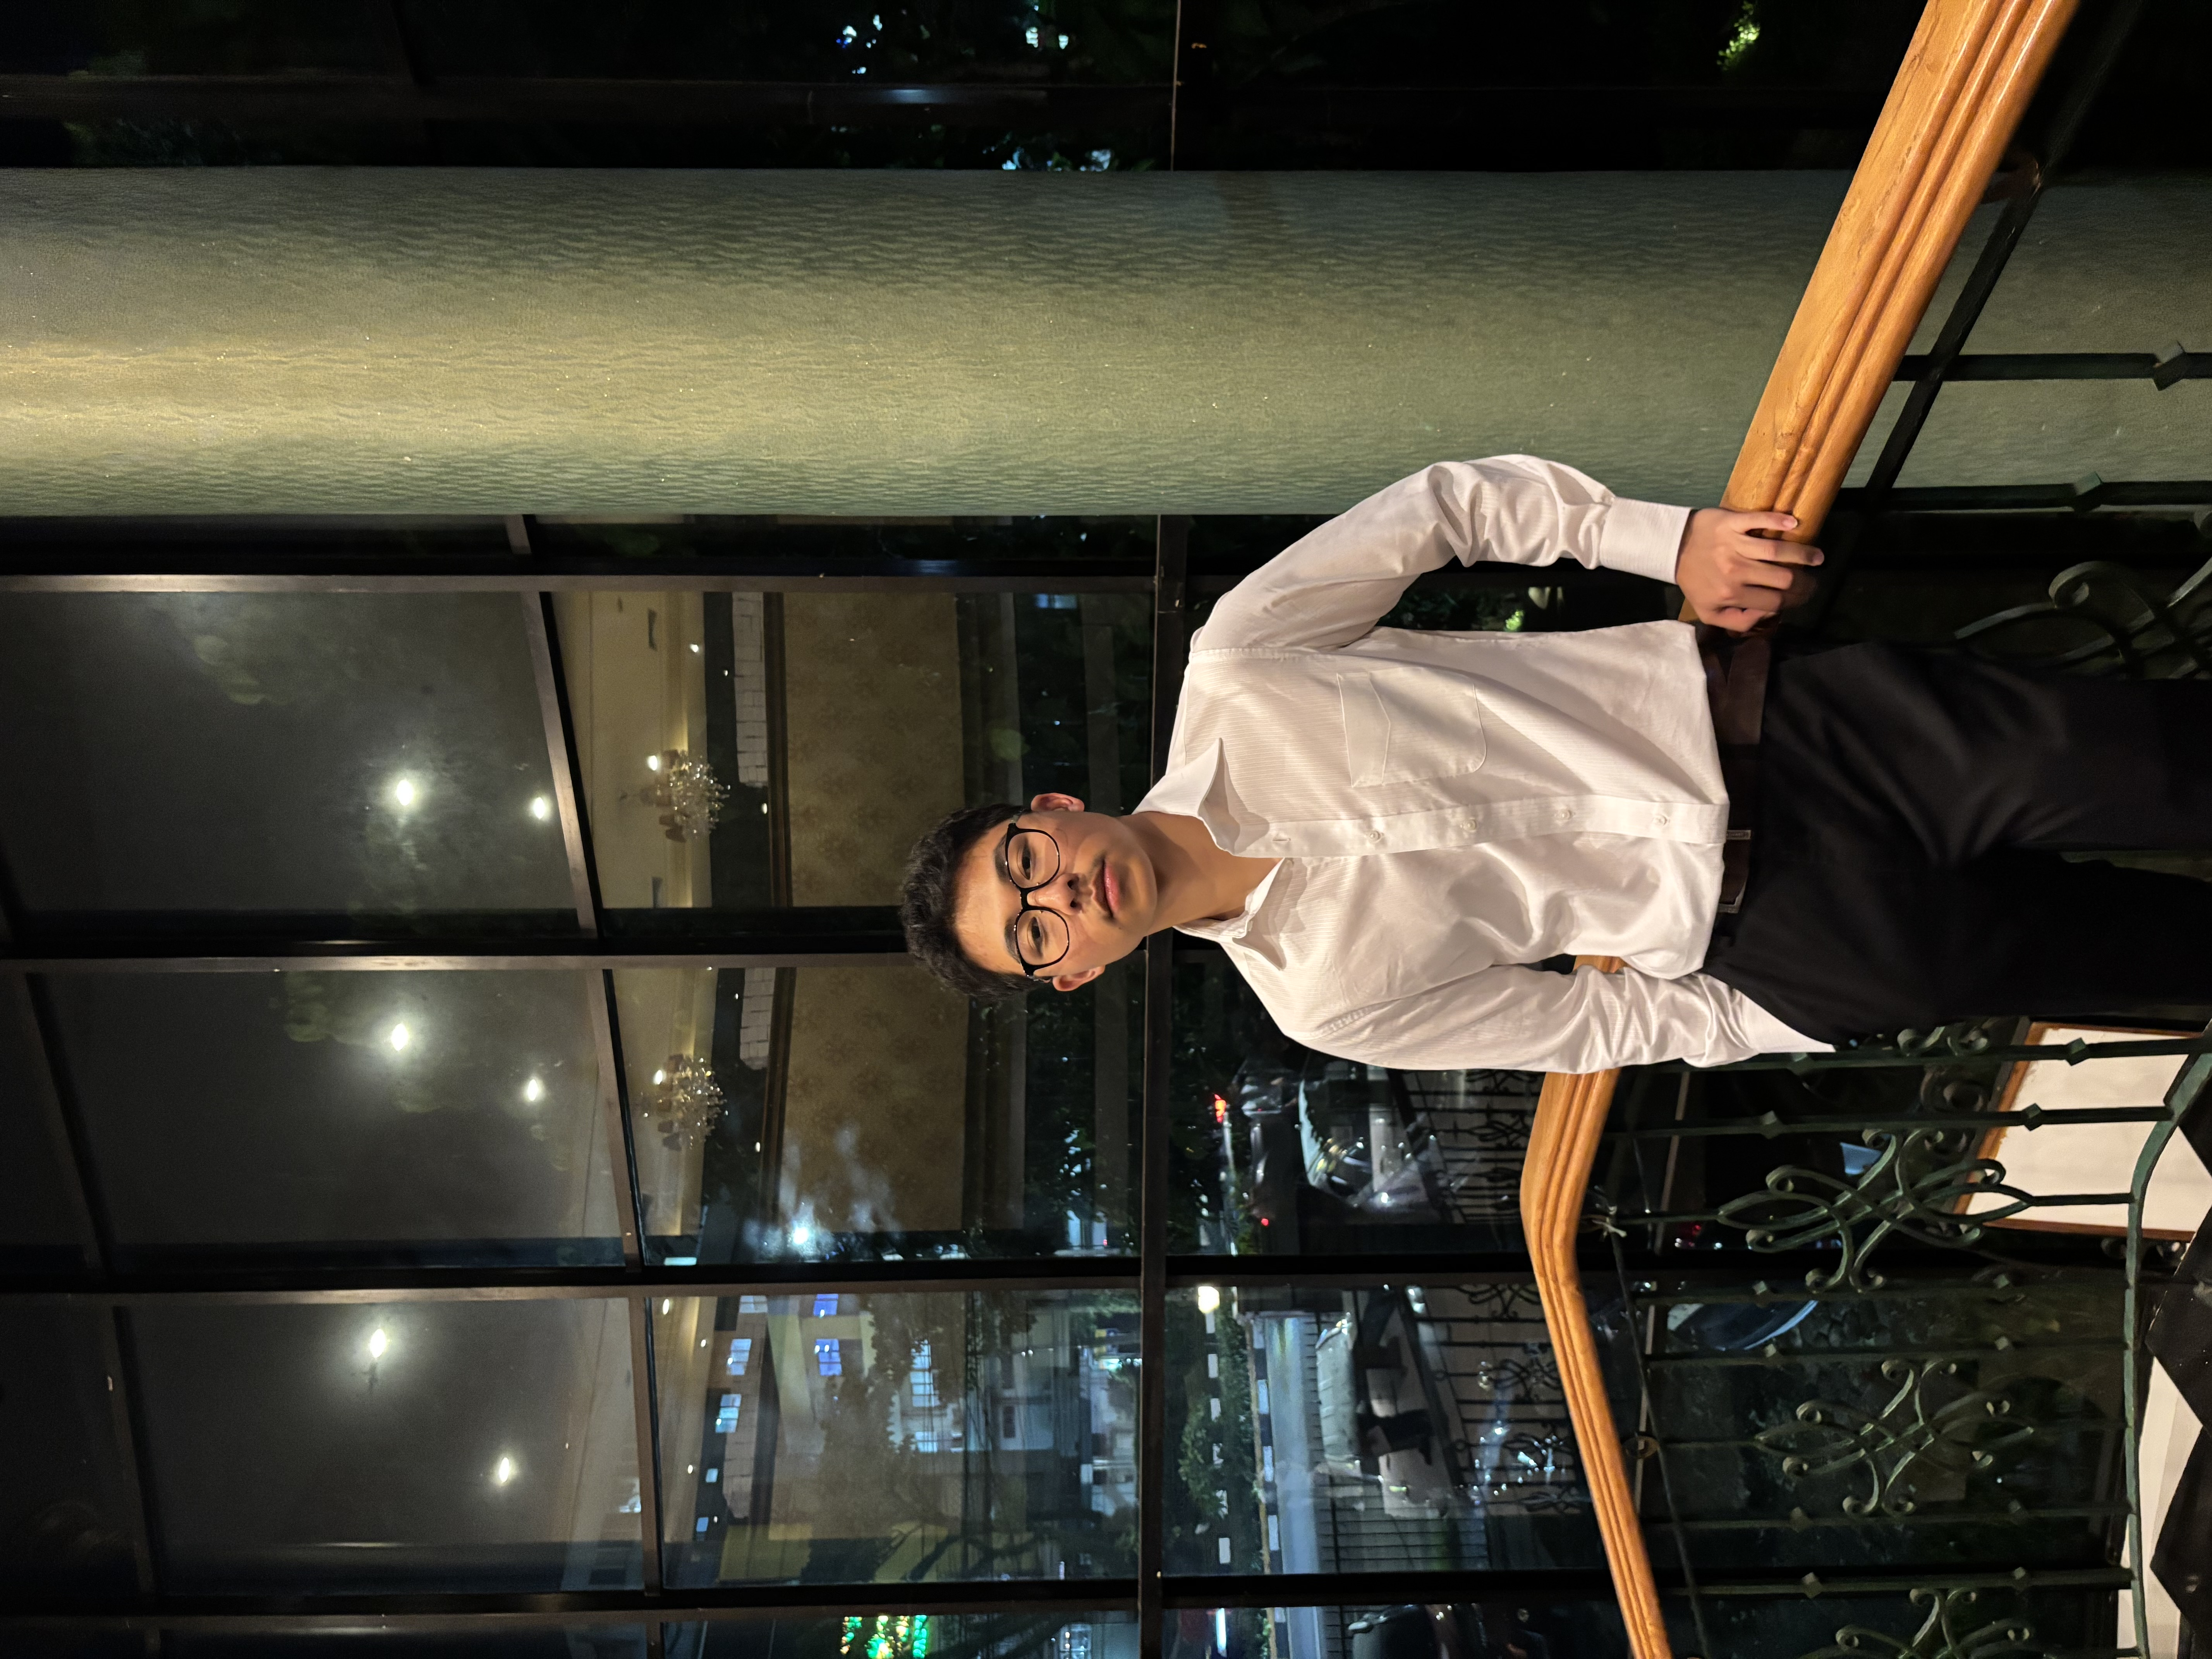
\includegraphics[width=1\linewidth,height=\textheight,keepaspectratio]{images/oks.jpg}

}

\caption{About Me}

\end{figure}%

Halo! Senang sekali Anda mampir!

Perkenalkan, saya Jonathan Kenan Budianto, atau panggil saja Kenan. Saya
adalah seorang pemimpi berusia 19 tahun dari Jakarta yang sedang memulai
salah satu petualangan paling seru dalam hidup: menjadi seorang
mahasiswa. Bagi saya, setiap hari adalah sebuah halaman baru yang siap
diisi dengan pembelajaran, tawa, dan tentu saja, cerita-cerita tak
terduga!

Saya tumbuh dalam kehangatan keluarga besar, di mana pintu rumah selalu
terbuka dan meja makan tak pernah sepi. Kakek dan nenek saya adalah
pahlawan saya; mereka mengajarkan sebuah pelajaran sederhana namun
sangat mendalam: bahwa kebaikan tidak mengenal batas, dan setiap orang
yang kita temui adalah bagian dari keluarga besar kita sendiri. Filosofi
inilah yang menjadi kompas hidup saya, sebuah pengingat untuk selalu
menyebarkan kepedulian dan membangun jembatan, bukan tembok.

Ada sebuah percikan semangat di dalam diri saya yang selalu menyala
paling terang ketika saya bisa menjadi bagian dari sesuatu yang lebih
besar. Saya sangat percaya pada kekuatan kolaborasi dan pemberdayaan.
Melihat sebuah ide tumbuh menjadi kenyataan, menyaksikan orang-orang di
sekitar saya mencapai potensi mereka, dan merasakan energi dari sebuah
komunitas yang bergerak bersama---itulah yang membuat saya bersemangat!
Visi saya sederhana: menggunakan setiap ilmu dan karakter yang saya
miliki untuk ikut serta membangun masyarakat yang lebih baik, lebih
adil, dan lebih sinergis.

Di sini, di ruang digital kecil ini, saya ingin mengajak Anda untuk
melihat dunia melalui mata saya. Ini bukan sekadar portofolio; ini
adalah kumpulan fragmen perjalanan saya---dari momen-momen penuh tawa,
pelajaran berharga, hingga impian-impian besar yang sedang saya kejar.

Jadi, mari kita mulai petualangan ini. Selamat menjelajah, dan saya
harap Anda menemukan sesuatu yang menginspirasi di sini!

\bookmarksetup{startatroot}

\chapter{UTS-1: Peta Pembentuk Diri}\label{uts-1-peta-pembentuk-diri}

Siapakah saya? Pertanyaan itu terdengar sederhana, namun jawabannya
adalah mozaik dari ribuan momen, perjumpaan, dan pembelajaran. Bagi
saya, Jonathan Kenan Budianto, ``diri'' bukanlah sesuatu yang statis,
melainkan sebuah cerita yang terus ditulis. Halaman ini adalah upaya
saya untuk membagikan beberapa bab terpenting dari cerita itu.

\subsection{Akar yang Menumbuhkan: Pelajaran dari
Rumah}\label{akar-yang-menumbuhkan-pelajaran-dari-rumah}

Saya percaya kita adalah cerminan dari cinta yang kita terima. Fondasi
cerita saya dibangun di rumah kakek dan nenek, sebuah tempat di mana
kepedulian bukanlah kewajiban, melainkan udara yang kami hirup setiap
hari. Mereka mengajarkan sebuah kebenaran universal: bahwa setiap orang
yang kita temui adalah keluarga, dan setiap interaksi adalah kesempatan
untuk berbagi kebaikan.

Pelajaran ini menanamkan sebuah nilai inti dalam diri saya:
\textbf{empati}. Bukan sekadar memahami, tetapi benar-benar merasakan
dan bertindak. Nilai inilah yang menjadi kompas saya dalam menavigasi
kompleksitas hidup dan hubungan antarmanusia.

\subsection{Dari Ilmu ke Aksi: Kesenangan dalam
Memberdayakan}\label{dari-ilmu-ke-aksi-kesenangan-dalam-memberdayakan}

Ada sebuah kepuasan yang tak ternilai ketika ilmu yang kita pelajari di
ruang kelas bisa bertransformasi menjadi aksi nyata di masyarakat. Saya
menemukan percikan kebahagiaan itu saat terlibat dalam berbagai
kegiatan, di mana saya bisa melihat langsung bagaimana sebuah ide dapat
menumbuhkan harapan dan bagaimana kolaborasi dapat menciptakan perubahan
yang lebih besar dari yang bisa kita bayangkan.

Bagi saya, ini adalah inti dari ``aktualisasi diri'': bukan tentang
menjadi yang terbaik, tetapi tentang memberikan yang terbaik dari diri
kita untuk lingkungan sekitar. Ini adalah proses tanpa akhir untuk
menjadi pribadi yang lebih kritis, peduli, dan terlibat dalam membentuk
masyarakat yang ideal---sebuah masyarakat yang sinergis dan didasari
oleh etika dan kebenaran.

\subsection{Visi ke Depan: Menjadi Penulis Cerita yang
Berdampak}\label{visi-ke-depan-menjadi-penulis-cerita-yang-berdampak}

Perjalanan ini masih panjang, dan saya tahu akan ada banyak bab baru
yang menanti. Visi saya ke depan sederhana: terus belajar, terus
bertumbuh, dan terus memanfaatkan setiap kesempatan untuk menerapkan
ilmu dan karakter demi kebaikan bersama.

Pada akhirnya, ``All About Me'' bukan hanya tentang siapa saya sekarang,
tetapi tentang siapa saya ingin menjadi: seseorang yang ceritanya dapat
membawa dampak positif bagi banyak orang.

\bookmarksetup{startatroot}

\chapter{UTS-2: Sebuah Melodi untuk Masa Lalu yang
Membentukku}\label{uts-2-sebuah-melodi-untuk-masa-lalu-yang-membentukku}

Ada kenangan yang begitu kuat hingga warnanya tak akan pernah pudar,
bahkan dalam lembaran foto hitam putih sekalipun. Musik, bagi saya,
adalah mesin waktu yang bisa membawa kembali kehangatan dari kenangan
itu. Lagu ini bukan sekadar lagu; ini adalah ucapan terima kasih saya
yang paling tulus untuk fondasi hidup yang telah diberikan.

\begin{center}\rule{0.5\linewidth}{0.5pt}\end{center}

\subsection{``Monokrom'' oleh Tulus}\label{monokrom-oleh-tulus}

\emph{Sebuah surat cinta untuk kakek, nenek, dan semua kebaikan yang
mereka tanamkan.}

Setiap kali mendengar lagu ini, saya seperti diajak kembali ke rumah
masa kecil saya. Tulus bernyanyi tentang ``lembaran foto hitam putih'',
dan saya teringat akan semua pelajaran tanpa kata yang saya terima dari
kakek dan nenek. Mereka mengajarkan bahwa inti dari hidup bukanlah apa
yang kita miliki, melainkan seberapa besar kepedulian yang kita bagikan.

Lirik ``Denganmu, gelap ku tak pernah kelabu'' adalah kalimat yang
paling tepat untuk menggambarkan peran mereka. Mereka adalah cahaya yang
memastikan bahwa perjalanan saya selalu dipenuhi warna harapan dan
kebaikan. Lagu ini adalah perayaan untuk masa lampau yang tidak akan
pernah hilang ditelan waktu, sebuah pengingat abadi akan akar dari mana
saya bertumbuh.

\url{https://www.youtube.com/watch?v=I-QQa_m_c8g}

\begin{quote}
\textbf{Lirik Lengkap ``Monokrom''}

Lembaran foto hitam putih Aku coba ingat lagi warna bajumu kala itu Kali
pertama di hidupku Manusia lain memelukku

Lembaran foto hitam putih Aku coba ingat lagi wangi rumah di sore itu
Kue cokelat dan susu Dan tiga bocah di selebar koran sore

Di mana pun kalian berada Kukirimkan terima kasih Untuk warna dalam
hidupku dan banyak kenangan indah Kau melukis aku

Lembaran foto hitam putih Kembali teringat malam kuhitung-hitung bintang
Saat mataku sulit tidur Suaramu buatku lelap

Di mana pun kalian berada Kukirimkan terima kasih Untuk warna dalam
hidupku dan banyak kenangan indah Kau melukis aku

Kita tak pernah tahu berapa lama kita diberi waktu Jika aku pergi lebih
dulu, jangan lupakan aku Ini lagu untukmu, ungkapan terima kasihku

Lembar monokrom hitam putih Aku coba ingat warna demi warna di hidupku
Tak akan ku mengenal cinta Bila bukan karena hati baikmu
\end{quote}

\bookmarksetup{startatroot}

\chapter{UTS-3 My Stories for You}\label{uts-3-my-stories-for-you}

A story about my oldest daughter
\href{https://azrl.wordpress.com/2020/07/18/gaun-pengantin-gladys/\#comment-28004}{Gaun
Pemngantin Gladys}

A message to my daughter
\href{https://azrl.wordpress.com/2021/10/06/the-child-who-learned-to-walk-at-the-disneyland/}{The
Child Who Learned to Walk at the Disneyland}

A story for my students
\href{https://azrl.wordpress.com/2008/04/21/fly-my-eagle-fly/}{Fly Eagle
Fly}

A (true) story for my teachers
\href{\%3Chttps://azrl.wordpress.com/2012/11/28/perginya-sang-mahaputera-dan-mahaguru-berkemeja-putih/}{Sang
Mahaguru, Sang Mahaputera}

Teasing story \url{https://www.youtube.com/watch?v=Dg_4PbBlBf4}

\bookmarksetup{startatroot}

\chapter{UTS-4 My SHAPE (Spiritual Gifts, Heart, Abilities, Personality,
Experiences)}\label{uts-4-my-shape-spiritual-gifts-heart-abilities-personality-experiences}

\begin{quote}
\textbf{Tujuan:} Merangkum rancangan diri (charter) agar saya melayani,
berkarya, dan memimpin secara paling selaras dengan karunia dan
pengalaman hidup saya. Dapat langsung ditempel ke halaman \textbf{UTS-4
--- My SHAPE} dan dipakai sebagai acuan aksi 90 hari.
\end{quote}

\section{\texorpdfstring{Sumber
\href{StrengthsProfile-Armein-Langi.pdf}{VIA
assessment}}{Sumber VIA assessment}}\label{sumber-via-assessment}

\section{0) Ringkasan 1 Halaman}\label{ringkasan-1-halaman}

\textbf{Peran Inti:} Profesor \& Elder --- perancang ekosistem
belajar-bernilai, pembimbing, dan pemimpin pelayanan komunitas.
\textbf{Misi:} Mengangkat kualitas hidup melalui \emph{smart
engineering} dan \emph{value-oriented education}, khususnya bagi
lansia/keluarga/komunitas (GRACE), serta pelayanan gerejawi yang
menumbuhkan kasih dan pengharapan. \textbf{Kekuatan Utama:} mengkonsep
sistem utuh, menulis \& mengajar, membangun jejaring, merancang
rubrik/alat evaluasi, menggerakkan proyek lintas-disiplin.
\textbf{Dampak yang Dituju:} karya, kurikulum, dan pelayanan yang
menumbuhkan karakter, keterampilan, serta kesejahteraan berkeadilan.

\textbf{Peta SHAPE (singkat):}

\begin{itemize}
\tightlist
\item
  \textbf{S --- Spiritual Gifts:} Teaching, Shepherding/Pastoring,
  Leadership, Wisdom/Discernment, Exhortation/Encouragement,
  Administration.
\item
  \textbf{H --- Heart (Minat \& Cinta Pelayanan):} pendidikan
  berorientasi nilai; kesejahteraan lansia \& keluarga (GRACE);
  pembinaan iman; menulis kisah/novel/lirik; rekayasa cerdas \& AI untuk
  kebaikan bersama; mentorship mahasiswa-dosen; penguatan jemaat.
\item
  \textbf{A --- Abilities (Kemampuan):} perancangan sistem (PSKVE/TISE),
  kurikulum \& rubrik, riset \& publikasi, menulis multi-format
  (Quarto/LaTeX), pemrograman (Python/R/Prolog/Modelica), komunikasi
  publik, memimpin kolaborasi.
\item
  \textbf{P --- Personality (Gaya Kepribadian Kerja):} strategis \&
  reflektif, berorientasi visi \& nilai, analitis-sistemik, kolaboratif,
  tenang dalam krisis, suka membangun standar \& alat.
\item
  \textbf{E --- Experiences (Pengalaman Kunci):} dosen \& peneliti
  lintas proyek (GRACE, Smart Engineering, pendidikan), Elder \&
  pengorganisasi jemaat, penulis kreatif, arsitek sistem pengetahuan
  (Obsidian/GitHub/Quarto), penggerak sarasehan \& penggalangan
  dukungan.
\end{itemize}

\begin{center}\rule{0.5\linewidth}{0.5pt}\end{center}

\section{1) S --- Spiritual Gifts (Karunia
Rohani)}\label{s-spiritual-gifts-karunia-rohani}

\begin{itemize}
\tightlist
\item
  \textbf{Teaching \& Wisdom/Discernment:} mengubah konsep kompleks
  menjadi peta belajar, rubrik, dan alat evaluasi yang memampukan.
\item
  \textbf{Shepherding/Pastoring \& Exhortation:} membimbing
  individu/kelompok dengan empati, meneguhkan, dan memberi arah.
\item
  \textbf{Leadership \& Administration:} merancang ekosistem
  (orang--proses--alat) dengan target berdampak dan terukur.
\end{itemize}

\textbf{Indikator Bukti:} silabus \& rubrik (II-2100/EL2007), naskah
pengajaran, bimbingan riset, modul/website kelas, program jemaat.

\begin{center}\rule{0.5\linewidth}{0.5pt}\end{center}

\section{2) H --- Heart (Minat, Nilai,
Kepedulian)}\label{h-heart-minat-nilai-kepedulian}

\begin{itemize}
\tightlist
\item
  Pendidikan yang \textbf{mencipta nilai} (CPMK↔rubrik↔artefak nyata).
\item
  \textbf{GRACE}: kualitas hidup lansia/keluarga melalui sistem dukung
  cerdas \& komunitas saling-melayani.
\item
  \textbf{Gereja \& Komunitas}: penguatan iman, kesalingan, dan
  pelayanan kasih.
\item
  \textbf{Kreativitas naratif}: kisah/novel/lirik sebagai sarana edukasi
  \& pengharapan.
\item
  \textbf{Rekayasa cerdas \& AI} untuk kemaslahatan.
\end{itemize}

\textbf{Masalah yang ingin dipecahkan:} kesenjangan antara
pengetahuan--karakter--aksi; pembelajaran kurang bermakna; layanan
komunitas belum terukur dampaknya.

\begin{center}\rule{0.5\linewidth}{0.5pt}\end{center}

\section{3) A --- Abilities (Kemampuan
Andal)}\label{a-abilities-kemampuan-andal}

\begin{itemize}
\tightlist
\item
  \textbf{Perancangan sistem} (PSKVE/TISE), \emph{value co‑creation},
  finansial rekayasa, desain instrumen penilaian.
\item
  \textbf{Kurikulum \& pedagogi}: CPMK↔rubrik↔tugas↔bukti; otomasi alur
  kerja (Python/Quarto/GitHub).
\item
  \textbf{Riset \& penulisan ilmiah}; \textbf{karya kreatif} (prosa,
  lirik, ceramah/khotbah).
\item
  \textbf{Teknis}: Python, R, Prolog (ontologi), Modelica, Quarto/LaTeX,
  Obsidian, GitHub, Graphviz.
\item
  \textbf{Komunikasi \& kepemimpinan}: orasi publik, fasilitasi
  sarasehan, negosiasi kolaborasi.
\end{itemize}

\begin{center}\rule{0.5\linewidth}{0.5pt}\end{center}

\section{4) P --- Personality (Gaya Kerja \&
Kolaborasi)}\label{p-personality-gaya-kerja-kolaborasi}

\begin{itemize}
\tightlist
\item
  \textbf{Strategis‑sistemik} (melihat gambaran besar, memetakan
  bagian-bagian).
\item
  \textbf{Reflektif \& nilai‑driven} (standar etis \& mutu).
\item
  \textbf{Kolaboratif} (membangun jejaring, memberi ruang tumbuh).
\item
  \textbf{Tenang‑tangguh} (fokus hasil jangka panjang).
\item
  \textbf{Pembelajar \& pembuat alat} (suka membuat template, rubrik,
  pipeline).
\end{itemize}

\begin{center}\rule{0.5\linewidth}{0.5pt}\end{center}

\section{5) E --- Experiences (Pengalaman
Pembentuk)}\label{e-experiences-pengalaman-pembentuk}

\begin{itemize}
\tightlist
\item
  \textbf{Akademik \& Riset:} merancang mata kuliah, SLR AI \&
  transformasi digital, proyek GRACE \& Smart Engineering.
\item
  \textbf{Pelayanan \& Organisasi:} Elder GKI, fasilitator sarasehan,
  penggalangan dukungan jemaat, pembinaan rohani.
\item
  \textbf{Kreasi Konten:} penulisan novel/khotbah/lirik; produksi materi
  ajar multi‑format.
\item
  \textbf{Infrastruktur Pengetahuan:} Obsidian--GitHub--Quarto, rubrik
  otomatis, bank soal.
\end{itemize}

\textbf{Pelajaran Inti:} integrasi iman--ilmu--nilai; sistem yang baik
melipatgandakan orang baik; narasi menggerakkan aksi.

\begin{center}\rule{0.5\linewidth}{0.5pt}\end{center}

\section{6) Piagam Diri (Self‑Charter)}\label{piagam-diri-selfcharter}

\textbf{Misi Hidup:} merancang dan menggerakkan ekosistem pembelajaran
\& pelayanan yang memerdekakan, bermakna, dan berkeadilan. \textbf{Nilai
Inti:} kasih, integritas, kebijaksanaan, keberanian, mutu, keberpihakan
pada yang lemah. \textbf{Peran Inti:} Perancang sistem
nilai‑pembelajaran; Pembimbing \& pengajar; Pemimpin pelayanan
komunitas. \textbf{Kompas Keputusan:} (1) Dampak pada manusia; (2)
Keselarasan nilai; (3) Keberlanjutan; (4) Kemampuan tim mengelola; (5)
Bukti terukur. \textbf{Janji Pelayanan:} hadir dengan empati, mendengar,
memberi arah praktis, membangun alat agar orang lain bertumbuh.
\textbf{Batasan:} menolak proyek yang mengabaikan martabat
manusia/etika; menjaga ritme kerja‑istirahat‑keluarga.

\begin{center}\rule{0.5\linewidth}{0.5pt}\end{center}

\section{7) Narasi 90 Detik (Elevator
Pitch)}\label{narasi-90-detik-elevator-pitch}

``Saya seorang profesor dan elder yang merancang ekosistem belajar dan
pelayanan berbasis nilai. Karunia saya mengajar, membimbing, dan
memimpin dengan pendekatan sistem: mengubah konsep besar menjadi peta,
rubrik, dan alat yang membuat orang bertumbuh. Hati saya pada pendidikan
bermakna, kesejahteraan lansia dan keluarga, serta penguatan jemaat.
Dengan pengalaman lintas riset, kurikulum, dan pelayanan, saya
menghubungkan ilmu, iman, dan aksi. Target saya sederhana: menghadirkan
karya dan komunitas yang saling menguatkan---di kelas, di gereja, dan di
masyarakat---agar lebih banyak orang hidup berkualitas, berpengharapan,
dan siap melayani.''

\begin{center}\rule{0.5\linewidth}{0.5pt}\end{center}

\section{8) Service‑Fit Map (Tempat Saya Paling
Berdampak)}\label{servicefit-map-tempat-saya-paling-berdampak}

\begin{itemize}
\tightlist
\item
  \textbf{Kampus:} perancangan kurikulum \& rubrik; mentorship riset;
  otomasi pipeline belajar; kuliah \& orasi.
\item
  \textbf{Jemaat:} pembinaan rohani \& khotbah; fasilitasi sarasehan;
  program lansia/keluarga (GRACE).
\item
  \textbf{Riset‑Inovasi:} desain platform nilai‑ciptakan (PSKVE);
  publikasi; konsorsium kolaborasi.
\item
  \textbf{Kreasi Naratif:} kisah/lirik sebagai media edukasi \&
  penguatan batin.
\end{itemize}

\begin{center}\rule{0.5\linewidth}{0.5pt}\end{center}

\section{9) Evidences (Artefak \&
Tautan)}\label{evidences-artefak-tautan}

\begin{quote}
Ganti tanda {[} {]} dengan tautan/berkas Anda.
\end{quote}

\begin{itemize}
\tightlist
\item[$\square$]
  Silabus \& rubrik II‑2100 / EL2007
\item[$\square$]
  Modul/website kelas \& bank soal
\item[$\square$]
  Khotbah/renungan \& materi sarasehan
\item[$\square$]
  Publikasi/SLR \& proposal riset (GRACE, dsb.)
\item[$\square$]
  Novel/lirik \& materi kreatif
\item[$\square$]
  Pipeline otomasi (Quarto/GitHub/Obsidian)
\end{itemize}

\begin{center}\rule{0.5\linewidth}{0.5pt}\end{center}

\section{10) Rencana Aksi 90 Hari
(SMART)}\label{rencana-aksi-90-hari-smart}

\begin{enumerate}
\def\labelenumi{\arabic{enumi}.}
\tightlist
\item
  \textbf{Rampungkan halaman UTS (KIPP/All‑About‑Me) end‑to‑end.}
  \emph{Outcome:} semua tugas berisi bukti + rubrik; \emph{Due:} T‑14
  hari.
\item
  \textbf{Mentor 3 tim mahasiswa menyusun artefak bernilai.}
  \emph{Outcome:} 3 proyek dengan metrik dampak; \emph{Due:} T‑45 hari.
\item
  \textbf{Pilot GRACE micro‑service di jemaat.} \emph{Outcome:} 1
  layanan kecil terukur (mis. pendampingan lansia); \emph{Due:} T‑90
  hari.
\item
  \textbf{Publikasi ringkas (working paper) integrasi
  iman--ilmu--nilai.} \emph{Outcome:} 1 naskah pra‑cetak; \emph{Due:}
  T‑75 hari.
\end{enumerate}

\begin{center}\rule{0.5\linewidth}{0.5pt}\end{center}

\section{11) SHAPE ↔ CPMK (Interpersonal \& Public
Communication)}\label{shape-cpmk-interpersonal-public-communication}

\begin{itemize}
\tightlist
\item
  \textbf{Self‑awareness \& refleksi (CPMK‑S):} dituangkan pada Piagam
  Diri \& Narasi 90 detik.
\item
  \textbf{Empati \& komunikasi etis (CPMK‑E):} Shepherding/Exhortation →
  khotbah, mentoring, review berempati.
\item
  \textbf{Storytelling \& presentasi (CPMK‑P):} Teaching + kreasi
  naratif → kuliah, cerita, lirik.
\item
  \textbf{Kolaborasi \& kepemimpinan (CPMK‑K):}
  Leadership/Administration → proyek riset/komunitas terukur.
\end{itemize}

\begin{center}\rule{0.5\linewidth}{0.5pt}\end{center}

\section{12) Self‑Assessment Rubrik UTS‑4 (isi
skormu)}\label{selfassessment-rubrik-uts4-isi-skormu}

\begin{longtable}[]{@{}
  >{\raggedright\arraybackslash}p{(\linewidth - 6\tabcolsep) * \real{0.3382}}
  >{\raggedright\arraybackslash}p{(\linewidth - 6\tabcolsep) * \real{0.4412}}
  >{\raggedleft\arraybackslash}p{(\linewidth - 6\tabcolsep) * \real{0.1471}}
  >{\raggedright\arraybackslash}p{(\linewidth - 6\tabcolsep) * \real{0.0735}}@{}}
\toprule\noalign{}
\begin{minipage}[b]{\linewidth}\raggedright
Kriteria
\end{minipage} & \begin{minipage}[b]{\linewidth}\raggedright
Deskripsi
\end{minipage} & \begin{minipage}[b]{\linewidth}\raggedleft
Skor (1--5)
\end{minipage} & \begin{minipage}[b]{\linewidth}\raggedright
Bukti
\end{minipage} \\
\midrule\noalign{}
\endhead
\bottomrule\noalign{}
\endlastfoot
Kelengkapan SHAPE & S‑H‑A‑P‑E jelas \& terisi & & \\
Koherensi Piagam Diri & misi‑nilai‑peran konsisten & & \\
Narasi 90 detik & ringkas, kuat, mengundang aksi & & \\
Evidence \& Aksi 90 hari & tautan bukti \& rencana SMART & & \\
\end{longtable}

\textbf{Total (maks 20):} {[} {]} \textbf{Tingkat:} ☐ A (≥85\%) ☐ B
(70--84\%) ☐ C (60--69\%) ☐ D (50--59\%) ☐ E (\textless50\%)

\begin{center}\rule{0.5\linewidth}{0.5pt}\end{center}

\section{13) Versi Ultra‑Ringkas (≤140
kata)}\label{versi-ultraringkas-140-kata}

``Saya profesor \& elder dengan karunia mengajar, membimbing, dan
memimpin secara sistemik. Hati saya pada pendidikan bernilai,
kesejahteraan lansia/keluarga (GRACE), dan penguatan jemaat. Kemampuan
saya merancang kurikulum, rubrik, dan alat otomasi belajar; menulis
ilmiah \& kreatif; serta menggerakkan kolaborasi. Pengalaman saya di
kampus, gereja, riset, dan kreasi konten mengajarkan integrasi
iman--ilmu--aksi. Misi saya menghadirkan ekosistem yang memerdekakan: di
kelas melalui pembelajaran bermakna; di jemaat melalui pelayanan kasih
yang terukur; dan di masyarakat melalui inovasi yang adil. Target 90
hari: menuntaskan artefak UTS, mementori 3 tim mahasiswa, memulai
layanan mikro GRACE, dan menerbitkan naskah ringkas.''

\section{Piagam Diri --- Armein Z. R.
Langi}\label{piagam-diri-armein-z.-r.-langi}

\textbf{Pernyataan Misi} Saya adalah insinyur-pendidik dan penulis yang
menyalakan sukacita belajar, menumbuhkan empati, dan merancang sistem
cerdas yang memuliakan Tuhan serta meningkatkan kualitas hidup keluarga,
kampus, dan komunitas. (Struktur mengikuti kerangka \emph{My
SHAPE}---Piagam Diri 1-halaman. )

\textbf{S --- Signature Strengths (inti kekuatan khas)} Humor,
Spiritualitas, Kreativitas, Suka Belajar, Keingintahuan, Pandangan
(wisdom/perspective), Bersyukur, Keadilan, Kecerdasan Sosial, Kejujuran,
Kepemimpinan. (Sumber: VIA Character Strengths Profile, 13 Okt 2025. )

\textbf{H --- Heart (nilai \& panggilan)} Empati sebagai kecerdasan
tertinggi; kebaikan lebih utama daripada sekadar pintar; pencarian ``The
True Reality''; sukacita hidup yang mengasihi; keluarga sebagai
ekosistem kasih. (Disimpulkan dari tulisan-tulisan Anda di blog:
\emph{Empati: Kecerdasan Tertinggi}; \emph{On Being Nice}; \emph{The
Truth, The True Reality}; tagline blog; catatan keluarga.
(\href{https://ii-2100.github.io/all-about-me/}{Armein Z. R. Langi in
the City of Eden}))

\textbf{A --- Aptitudes \& Acquired Skills (bakat \& keterampilan
kunci)} Perancangan \& penelitian sistem/komputasi (speech compression,
FPGA), rekayasa \& kurikulum, kepemimpinan akademik, penulisan \&
penceritaan, fasilitasi pembelajaran, sistem \& organisasi. (Contoh
teknis: riset speech compression \& desain kontrol prosesor pada awal
karier.
(\href{https://ii-2100.github.io/all-about-me/My_Song_for_You/index.html}{Armein
Z. R. Langi in the City of Eden}))

\textbf{P --- Personality (gaya kerja yang menonjol)}
Reflektif-analitis, empatik-inklusif, visioner, pembelajar antusias,
kolaboratif; berpihak pada keadilan \& integritas. (Disintesis dari pola
kekuatan VIA dan tema tulisan Anda. )

\textbf{E --- Experiences (jejak pembentuk identitas)}

\begin{itemize}
\tightlist
\item
  \textbf{Ketangguhan pribadi} --- ``The Child Who Learned to Walk at
  the Disneyland'': ketekunan, berjalan dalam dingin, terus melangkah
  menuju tujuan.
  (\href{https://ii-2100.github.io/all-about-me/My_Stories_for_You/index.html}{Armein
  Z. R. Langi in the City of Eden})
\item
  \textbf{Lompatan kompetensi awal} --- perjalanan riset: software
  speech compression jadi dalam 3 bulan; desain chip kontrol di Xilinx
  FPGA; menulis paper.
  (\href{https://ii-2100.github.io/all-about-me/My_Song_for_You/index.html}{Armein
  Z. R. Langi in the City of Eden})
\item
  \textbf{Keluarga \& komunitas} --- keluarga besar sebagai sumber
  nilai, pelayanan, dan sukacita.
  (\href{https://ii-2100.github.io/all-about-me/My_Shapes/index.html}{Armein
  Z. R. Langi in the City of Eden})
\item
  \textbf{Standar keunggulan} --- sensibilitas benchmarking sains \&
  pendidikan (refleksi tentang Caltech).
  (\href{https://ii-2100.github.io/all-about-me/My_Personal_Reviews/index.html}{Armein
  Z. R. Langi in the City of Eden})
\end{itemize}

\textbf{Janji Praktis (Operating Principles)}

\begin{enumerate}
\def\labelenumi{\arabic{enumi}.}
\tightlist
\item
  \emph{People first with empathy} • 2) \emph{Truth-seeking with
  humility} • 3) \emph{Design for value \& justice} • 4) \emph{Teach
  what I practice, practice what I teach} • 5) \emph{Joyful learning,
  faithful living}. (Kerangka dan cara merangkum diadaptasi dari
  \emph{My SHAPE Toolkit}. )
\end{enumerate}

\begin{center}\rule{0.5\linewidth}{0.5pt}\end{center}

\section{Narasi Diri (versi 90 detik)}\label{narasi-diri-versi-90-detik}

Saya Armein---insinyur, pendidik, dan penulis---yang percaya bahwa
pengetahuan hanya bermakna bila melahirkan kasih dan keadilan. Kekuatan
saya adalah \textbf{spiritualitas yang membumi, kreativitas rekayasa,
dan kegembiraan belajar tanpa henti}, yang saya pakai untuk menyalakan
semangat orang lain.

Perjalanan saya ditempa oleh pengalaman yang mengajarkan
\textbf{ketekunan}---mulai dari ``berjalan dalam dingin'' hingga tuntas
menyelesaikan riset komputasi dan merancang sistem sejak awal karier.
Keluarga dan komunitas menjadi ekosistem kasih tempat saya belajar bahwa
\textbf{kebaikan lebih tinggi nilainya daripada sekadar pintar} dan
\textbf{empati adalah kecerdasan tertinggi}.
(\href{https://ii-2100.github.io/all-about-me/My_Stories_for_You/index.html}{Armein
Z. R. Langi in the City of Eden})

Ke depan, saya ingin terus \textbf{mendesain lingkungan belajar dan
sistem cerdas} yang memuliakan Tuhan dan membawa berkat
nyata---membentuk insan pembelajar yang jujur, adil, dan penuh
syukur---seraya menjaga sukacita: \emph{joy of loving and exciting
life}.
(\href{https://ii-2100.github.io/all-about-me/My_Stories_for_You/index.html}{Armein
Z. R. Langi in the City of Eden})

\begin{center}\rule{0.5\linewidth}{0.5pt}\end{center}

\section{Narasi Diri (versi panjang, 3--5
paragraf)}\label{narasi-diri-versi-panjang-35-paragraf}

\textbf{Kini.} Saya mengabdikan diri sebagai insinyur-pendidik yang
merancang pengalaman belajar dan sistem cerdas agar manusia bertumbuh
utuh: cakap teknis, peka nurani, dan gembira belajar. Kekuatan
saya---spiritualitas, kreativitas, suka belajar, keingintahuan,
perspektif, keadilan, dan kepemimpinan---mengarahkan cara saya memimpin,
mengajar, dan menulis.

\textbf{Dulu---titik balik.} Saya belajar bahwa langkah kecil yang
konsisten mengalahkan rintangan besar: berjalan sendirian dalam
dingin---secara harfiah dan metaforis---membentuk ketahanan batin. Di
laboratorium, saya menuntaskan perangkat lunak \textbf{speech
compression} dalam waktu singkat dan merancang \textbf{control unit}
berbasis FPGA, lalu menulis paper pertama---momen yang mengajarkan
disiplin, standar mutu, dan keberanian intelektual.
(\href{https://ii-2100.github.io/all-about-me/My_Stories_for_You/index.html}{Armein
Z. R. Langi in the City of Eden})

\textbf{Nilai yang saya pegang.} Saya memilih \textbf{kebaikan} di atas
sekadar \textbf{kepintaran}, menempatkan \textbf{empati} sebagai
kecerdasan tertinggi, dan mengejar \textbf{kebenaran sebagai realitas
yang sesungguhnya}. Keluarga besar meneguhkan panggilan itu---rumah
sebagai laboratorium kasih dan keadilan.
(\href{https://azrl.wordpress.com/2010/01/09/on-being-nice/?utm_source=chatgpt.com}{Armein
Z. R. Langi in the City of Eden})

\textbf{Ke depan.} Dengan kerangka \textbf{My SHAPE}, saya terus
menyelaraskan kekuatan, nilai, keterampilan, gaya kerja, dan pengalaman
untuk merancang program, riset, dan karya tulis yang berdampak---agar
teknologi menjadi pelayan kemanusiaan, dan setiap ruang belajar menjadi
\emph{City of Eden}: tempat sukacita, kasih, dan keunggulan bertemu.

\bookmarksetup{startatroot}

\chapter{UTS-5 My Personal Reviews}\label{uts-5-my-personal-reviews}

Berikut cara saya melakukan review: mengguan chatGPT, saya mengattach
\href{skor_uts.pdf}{file promt ChatGPT}, disertai perintah :``self
assess uts-1 sanpai uts-5 dari URL
`https://ii-2100.github.io/all-about-me/'\,''

ChatGPT melakukan self-assessment UTS-1 s.d. UTS-5 langsung dari laman
yang Anda berikan dan menilai memakai rubrik tugas UTS (skala 1--5 per
kriteria). Rekap skor siap diunduh sebagai CSV:
\href{sandbox:/mnt/data/UTS_self_assessment.csv}{Download CSV
ringkasan}.

\bookmarksetup{startatroot}

\chapter{Hasil Self-Assessment UTS (URL:
ii-2100.github.io/all-about-me)}\label{hasil-self-assessment-uts-url-ii-2100.github.ioall-about-me}

\section{Identifikasi}\label{identifikasi}

\begin{itemize}
\tightlist
\item
  Nama \& NIM penulis: \textbf{Armein Z. R. Langi -- 131902360} (tertera
  di halaman depan portofolio).
  (\href{https://ii-2100.github.io/all-about-me/}{II 2100})
\item
  Penilai: \textbf{Self-assessment (Armein Z. R. Langi)}
\item
  Catatan cakupan: halaman beranda memuat ``About Me''; navigasi ke ``My
  Songs for You'', ``My Stories for You'', ``My Shapes'', dan ``My
  Personal Reviews'' tersedia.
  (\href{https://ii-2100.github.io/all-about-me/}{II 2100})
\end{itemize}

\section{Tinjauan Umum}\label{tinjauan-umum}

\begin{itemize}
\tightlist
\item
  \textbf{UTS-1 (All About Me)} hadir di beranda (``Selamat Berjumpa /
  About Me''). Isi memperkenalkan identitas dan latar personal secara
  padat. (\href{https://ii-2100.github.io/all-about-me/}{II 2100})
\item
  \textbf{UTS-2 (My Songs for You)} memuat judul karya dan tautan audio,
  namun lirik/isi tidak ditampilkan di halaman (file audio tidak bisa
  saya akses dari sini), sehingga penilaian konten terbatas pada
  kelengkapan presentasi.
  (\href{https://ii-2100.github.io/all-about-me/My_Song_for_You/index.html}{II
  2100})
\item
  \textbf{UTS-3 (My Stories for You)} berisi tautan ke beberapa cerita;
  konten naratif kuat, terutama pada kisah keluarga ``Gaun Pengantin
  Gladys'' serta kisah inspiratif lainnya.
  (\href{https://ii-2100.github.io/all-about-me/My_Stories_for_You/index.html}{II
  2100})
\item
  \textbf{UTS-4 (My SHAPE)} saat ini halaman kosong/tanpa isi, hanya
  navigasi.
  (\href{https://ii-2100.github.io/all-about-me/My_Shapes/index.html}{II
  2100})
\item
  \textbf{UTS-5 (My Personal Reviews)} berisi metode/tautan panduan
  review, namun belum ada contoh \textbf{review personal} yang lengkap
  terhadap sebuah pesan/teks.
  (\href{https://ii-2100.github.io/all-about-me/My_Personal_Reviews/index.html}{II
  2100})
\end{itemize}

\begin{center}\rule{0.5\linewidth}{0.5pt}\end{center}

\section{Tinjauan Spesifik + Skor
(1--5)}\label{tinjauan-spesifik-skor-15}

\subsection{UTS-1 --- All About Me (di
beranda)}\label{uts-1-all-about-me-di-beranda}

\textbf{Skor per kriteria:} Orisinalitas \textbf{3}, Keterlibatan
\textbf{3}, Humor \textbf{1}, Wawasan/Insight \textbf{3} → \textbf{Total
10/20 (50\%)}. \textbf{Alasan singkat:} Perkenalan diri faktual dan
jelas, namun gaya masih informatif ketimbang naratif (minim humor dan
moment ``hook''). (\href{https://ii-2100.github.io/all-about-me/}{II
2100}) \textbf{Saran perbaikan:} Buka dengan anekdot pribadi (1--2
paragraf) yang ``mengikat'' (mis. titik balik karier/keluarga),
tambahkan satu momen humor ringan, lalu tutup dengan refleksi singkat
tentang nilai/visi diri agar aspek insight naik.

\subsection{UTS-2 --- My Songs for You}\label{uts-2-my-songs-for-you}

\textbf{Skor per kriteria:} Orisinalitas \textbf{2}, Keterlibatan
\textbf{2}, Humor \textbf{1}, Inspirasi \textbf{2} → \textbf{Total 7/20
(35\%)}. \textbf{Alasan singkat:} Halaman menampilkan judul lagu ``River
in my Mind'', ``Heaven on Earth'', namun tanpa lirik/cerita di balik
lagu sehingga sulit menilai aspek pesan, humor, dan inspirasi.
(\href{https://ii-2100.github.io/all-about-me/My_Song_for_You/index.html}{II
2100}) \textbf{Saran perbaikan:} Tambahkan lirik lengkap, 1 paragraf
cerita proses kreatif, dan 2--3 kalimat ``pesan untukmu'' agar inspirasi
terbaca; sertakan player/tautan yang dapat diputar langsung + fallback
transkrip.

\subsection{UTS-3 --- My Stories for
You}\label{uts-3-my-stories-for-you-1}

\textbf{Skor per kriteria:} Orisinalitas \textbf{5}, Keterlibatan
\textbf{5}, Pengembangan Narasi \textbf{4}, Inspirasi \textbf{5} →
\textbf{Total 19/20 (95\%)}. \textbf{Alasan singkat:} Cerita ``Gaun
Pengantin Gladys'' dkk sangat personal, emosional, dan inspiratif; ritme
bertutur hidup serta detail situasional kuat (konten ramu unsur
penebusan/keluarga/iman).
(\href{https://ii-2100.github.io/all-about-me/My_Stories_for_You/index.html}{II
2100}) \textbf{Saran perbaikan:} Tambah ``lead'' 2--3 kalimat yang
merangkum pesan kunci tiap cerita; akhiri dengan ajakan/refleksi 1--2
kalimat agar resonansi ke pembaca makin jelas.

\subsection{UTS-4 --- My SHAPE}\label{uts-4-my-shape}

\textbf{Skor per kriteria:} Orisinalitas \textbf{1}, Keterlibatan
\textbf{1}, Pengembangan \textbf{1}, Inspirasi \textbf{1} →
\textbf{Total 4/20 (20\%)}. \textbf{Alasan singkat:} Konten belum
tersedia.
(\href{https://ii-2100.github.io/all-about-me/My_Shapes/index.html}{II
2100}) \textbf{Saran perbaikan (prioritas):}

\begin{enumerate}
\def\labelenumi{\arabic{enumi}.}
\tightlist
\item
  Tampilkan rekap SHAPE (Spiritual gifts, Heart, Abilities, Personality,
  Experiences) dalam 1 tabel ringkas + 3--5 butir bukti;
\item
  Narasikan 2 pengalaman kunci (±150 kata/each) yang menunjukkan
  ``signature strengths'';
\item
  Tutup dengan 3 rencana aksi konkret (who/what/when).
\end{enumerate}

\subsection{UTS-5 --- My Personal
Reviews}\label{uts-5-my-personal-reviews-1}

\textbf{Skor per kriteria:} Pemahaman Konsep \textbf{2}, Analisis Kritis
\textbf{1}, Argumentasi (Logos) \textbf{1}, Etos \& Empati \textbf{2},
Rekomendasi \textbf{1} → \textbf{Total 7/25 (28\%)}. \textbf{Alasan
singkat:} Halaman berisi metode cara menilai, tetapi \textbf{belum ada}
contoh \textbf{review personal} yang lengkap terhadap sebuah pesan/teks
sehingga aspek analisis-argumentasi tak terbaca.
(\href{https://ii-2100.github.io/all-about-me/My_Personal_Reviews/index.html}{II
2100}) \textbf{Saran perbaikan:} Pilih 1 karya personal (mis.
UTS-1/2/3), tulis review 400--600 kata: ringkas pesan, nilai dengan
rubrik, berikan 2--3 bukti kutipan, evaluasi etos/empati, lalu tutup
dengan rekomendasi perbaikan spesifik.

\begin{center}\rule{0.5\linewidth}{0.5pt}\end{center}

\section{Rekap Skor (ringkas)}\label{rekap-skor-ringkas}

\begin{itemize}
\tightlist
\item
  \textbf{UTS-1:} 10/20 → \textbf{50\%}
\item
  \textbf{UTS-2:} 7/20 → \textbf{35\%}
\item
  \textbf{UTS-3:} 19/20 → \textbf{95\%}
\item
  \textbf{UTS-4:} 4/20 → \textbf{20\%}
\item
  \textbf{UTS-5:} 7/25 → \textbf{28\%}
\end{itemize}

CSV lengkap sudah saya siapkan untuk dokumentasi dan olah lanjut:
\href{sandbox:/mnt/data/UTS_self_assessment.csv}{Download CSV
ringkasan}.

\section{Langkah Perbaikan Cepat (prioritas 1
minggu)}\label{langkah-perbaikan-cepat-prioritas-1-minggu}

\begin{enumerate}
\def\labelenumi{\arabic{enumi}.}
\tightlist
\item
  \textbf{Lengkapi UTS-4 (My SHAPE)} sesuai saran di atas;
\item
  \textbf{Tambahkan lirik + sinopsis} untuk tiap lagu di UTS-2 agar bisa
  dinilai isi/inspirasinya;
\item
  \textbf{Tulis 1 review personal penuh} (UTS-5) memakai rubrik (pilih
  salah satu karya Anda sendiri sebagai objek);
\item
  Revisi UTS-1 dengan pembuka anekdot + refleksi nilai diri.
\end{enumerate}

Jika Anda mau, saya bisa bantu merapikan UTS-4 (tabel SHAPE + narasi)
dan membuat kerangka cepat untuk \textbf{review} di UTS-5 dari salah
satu karya Anda.

\bookmarksetup{startatroot}

\chapter{UAS-1 My Concepts}\label{uas-1-my-concepts}

Mau hidup epik ? \href{lifestory.pdf}{Write your Life Story}

Apa itu berkonsep?

\url{https://youtu.be/QVfUlVBO80U?si=yM6q_rwV9rcDBbu7}

\bookmarksetup{startatroot}

\chapter{UAS-3 My Opinions}\label{uas-3-my-opinions}

SApa itu beropini? \href{BM\%20Opini.mp4}{Opini Berpengaruh}

Bagiamana menjaadi menarik? \href{./Interesting.mp4}{Menjadi Menarik}

\bookmarksetup{startatroot}

\chapter{UAS-3 My Innovations}\label{uas-3-my-innovations}

\bookmarksetup{startatroot}

\chapter{UAS-4 My Knowledge}\label{uas-4-my-knowledge}

Cara saya mengkomunikasikan sebuah pengatahuan sebagai petunjuk bagi
orang lain 1) saya tulis
\href{Rekomendasi\%20Presentasi\%20Efektif(Contoh\%20Makalah).pdf}{makalah
sebagai bahan utama} 2) lalu saya buat
\href{Contoh\%20Transkrip\%20Presentasi.pdf}{transkrip ucapan lisan} 3)
kemudian saya kembangkan
\href{Rekomendasi\%20Presentasi\%20(Contoh\%20Slides).pdf}{slide
pendukung trnsskrip} 4) lalu saya memproduksivideo audio visual
\url{https://youtu.be/ZbghfMvnPZc} \url{https://youtu.be/ZbghfMvnPZc}

\bookmarksetup{startatroot}

\chapter{UAS-5 My Professional
Reviews}\label{uas-5-my-professional-reviews}

Untuk melAkukan review, seperti pada
\href{../My_Personal_Reviews/Doc.5.Mengevaluasi-Esai-Berdasarkan-Rubrik.pdf}{pendekatan
AI}, kita membutuhkan rubrik

\bookmarksetup{startatroot}

\chapter{Summary}\label{summary}

In summary, this book has no content whatsoever.

\bookmarksetup{startatroot}

\chapter*{References}\label{references}
\addcontentsline{toc}{chapter}{References}

\markboth{References}{References}

\phantomsection\label{refs}




\end{document}
